%; whizzy paragraph -pdf xpdf -latex ./whizzypdfptex.sh
%; whizzy-paragraph "^\\\\begin{frame}\\|\\\\emtext"
% latex beamer presentation.
% platex, latex-beamer でコンパイルすることを想定。 

%     Tokyo Debian Meeting resources
%     Copyright (C) 2012 Junichi Uekawa

%     This program is free software; you can redistribute it and/or modify
%     it under the terms of the GNU General Public License as published by
%     the Free Software Foundation; either version 2 of the License, or
%     (at your option) any later version.

%     This program is distributed in the hope that it will be useful,
%     but WITHOUT ANY WARRANTY; without even the implied warreanty of
%     MERCHANTABILITY or FITNESS FOR A PARTICULAR PURPOSE.  See the
%     GNU General Public License for more details.

%     You should have received a copy of the GNU General Public License
%     along with this program; if not, write to the Free Software
%     Foundation, Inc., 51 Franklin St, Fifth Floor, Boston, MA  02110-1301 USA

\documentclass[cjk,dvipdfmx,12pt]{beamer}
\usetheme{Tokyo}
\usepackage{monthlypresentation}

%  preview (shell-command (concat "evince " (replace-regexp-in-string "tex$" "pdf"(buffer-file-name)) "&")) 
%  presentation (shell-command (concat "xpdf -fullscreen " (replace-regexp-in-string "tex$" "pdf"(buffer-file-name)) "&"))
%  presentation (shell-command (concat "evince " (replace-regexp-in-string "tex$" "pdf"(buffer-file-name)) "&"))

%http://www.naney.org/diki/dk/hyperref.html
%日本語EUC系環境の時
\AtBeginDvi{\special{pdf:tounicode EUC-UCS2}}
%シフトJIS系環境の時
%\AtBeginDvi{\special{pdf:tounicode 90ms-RKSJ-UCS2}}

\newenvironment{commandlinesmall}%
{\VerbatimEnvironment
  \begin{Sbox}\begin{minipage}{1.0\hsize}\begin{fontsize}{8}{8} \begin{BVerbatim}}%
{\end{BVerbatim}\end{fontsize}\end{minipage}\end{Sbox}
  \setlength{\fboxsep}{8pt}
% start on a new paragraph

\vspace{6pt}% skip before
\fcolorbox{dancerdarkblue}{dancerlightblue}{\TheSbox}

\vspace{6pt}% skip after
}
%end of commandlinesmall

\title{東京エリアDebian勉強会}
\subtitle{第121回 2014年12月度}
\author{野島貴英}
\date{2014年12月20日}
\logo{
\includegraphics[width=8cm]{image200607/openlogo-light.eps}}

\begin{document}

\begin{frame}
\titlepage{}
\end{frame}

\begin{frame}{設営準備にご協力ください。}
会場設営よろしくおねがいします。
\end{frame}

\begin{frame}{Agenda}
 \begin{minipage}[t]{0.45\hsize}
  \begin{itemize}
   \item 注意事項
	 \begin{itemize}
	  \item 写真はセミナールーム内のみ可です。
          \item 出入りは自由でないので、もし外出したい方は、野島まで一声くださいませ。
	 \end{itemize}
   \item 事前課題発表
  \end{itemize}
 \end{minipage} 
 \begin{minipage}[t]{0.45\hsize}
  \begin{itemize}
   \item 最近あったDebian関連のイベント報告
	 \begin{itemize}
	  \item 第120回 東京エリアDebian勉強会
	 \end{itemize}
   \item Debian Trivia Quiz
   \item DebianとFedoraでパッケージをリリースするまでの話
   \item DebianからみたLinux Mint
   \item 今後のイベント
   \item 今日の宴会場所
  \end{itemize}
 \end{minipage}
\end{frame}

\section{事前課題}
\emtext{事前課題}
{\footnotesize
\begin{prework}{ henrich }
  \begin{enumerate}
  \item Q.$B$I$3$G:#2s$NJY6/2q$N3+:E$rCN$j$^$7$?$+!)(B\\
    A. $BM'C#$dCN$j9g$$$+$iD>@\(B
  \item Q.$B2?$K$D$$$FJ9$-$?$$!?;22C<T$HOC$r$7$?$$$G$9$+!)(B\\
    A. \@kenhys$B$5$s$NOC$,3Z$7$_$G$9!*(B :)
  \item Q.hack time$B$K2?$r$7$^$9$+!)(B\\
    A. ($B2sEz$J$7(B)
  \end{enumerate}
\end{prework}

\begin{prework}{ $BLnEg(B }
  \begin{enumerate}
  \item Q.$B$I$3$G:#2s$NJY6/2q$N3+:E$rCN$j$^$7$?$+!)(B\\
    A. $B$=$NB>(B (Google$B8!:w%(%s%8%s$N8!:w7k2L$+$i(B)
  \item Q.$B2?$K$D$$$FJ9$-$?$$!?;22C<T$HOC$r$7$?$$$G$9$+!)(B\\
    A. $B$$$m$$$m$H!#;22C<T$H!#(B
  \item Q.hack time$B$K2?$r$7$^$9$+!)(B\\
    A. RC$BDY$7$H$+!"K]Lu$H$+!#(BRC$B$O(B\url{https://bugs.debian.org/release-critical/}$B;2>H!#(B
  \end{enumerate}
\end{prework}

\begin{prework}{ knok }
  \begin{enumerate}
  \item Q.$B$I$3$G:#2s$NJY6/2q$N3+:E$rCN$j$^$7$?$+!)(B\\
    A. Debian JP$B$N%a!<%j%s%0%j%9%H(B
  \item Q.$B2?$K$D$$$FJ9$-$?$$!?;22C<T$HOC$r$7$?$$$G$9$+!)(B\\
    A. key sign$B$d$j$^$9(B
  \item Q.hack time$B$K2?$r$7$^$9$+!)(B\\
    A. $B$$$/$D$+$N%=!<%9$N<L7P$H!"$G$-$l$P(BK\&R$B%9%?%$%k$NGS=|(B
  \end{enumerate}
\end{prework}

\begin{prework}{ koedoyoshida }
  \begin{enumerate}
  \item Q.$B$I$3$G:#2s$NJY6/2q$N3+:E$rCN$j$^$7$?$+!)(B\\
    A. Debian JP$B$N%a!<%j%s%0%j%9%H(B
  \item Q.$B2?$K$D$$$FJ9$-$?$$!?;22C<T$HOC$r$7$?$$$G$9$+!)(B\\
    A. $B%Q%C%1!<%8%s%0(B
  \item Q.hack time$B$K2?$r$7$^$9$+!)(B\\
    A. $B$^$C$?$j%a%s%F%J%s%9(B or $BK]Lu(B
  \end{enumerate}
\end{prework}

\begin{prework}{ kenhys }
  \begin{enumerate}
  \item Q.$B$I$3$G:#2s$NJY6/2q$N3+:E$rCN$j$^$7$?$+!)(B\\
    A. Twitter (@debianjp)
  \item Q.$B2?$K$D$$$FJ9$-$?$$!?;22C<T$HOC$r$7$?$$$G$9$+!)(B\\
    A. $B$f$/$f$/$O(BDebian$B$K0lK\2=$7$?$$$1$I2aEO4|$J$?$a(Bupstream$B$G(Bdebian,ubuntu$B8~$1$K%Q%C%1!<%8$rDs6!$7$F$$$k?M$N(Bdebian/$B4IM}=QE*$J%;%_%J!<$,J9$-$?$$(B
  \item Q.hack time$B$K2?$r$7$^$9$+!)(B\\
    A. porterbox$B$,$i$_$N2?$+(B
  \end{enumerate}
\end{prework}

\begin{prework}{ wbcchsyn }
  \begin{enumerate}
  \item Q.$B$I$3$G:#2s$NJY6/2q$N3+:E$rCN$j$^$7$?$+!)(B\\
    A. $BM'C#$dCN$j9g$$$+$iD>@\(B
  \item Q.$B2?$K$D$$$FJ9$-$?$$!?;22C<T$HOC$r$7$?$$$G$9$+!)(B\\
    A. $B:G6a$N>u67$K$D$$$F!">pJs8r49(B
  \item Q.hack time$B$K2?$r$7$^$9$+!)(B\\
    A. Debian $B$N3+H/4D6-9=C[(B
  \end{enumerate}
\end{prework}

\begin{prework}{ zinrai }
  \begin{enumerate}
  \item Q.$B$I$3$G:#2s$NJY6/2q$N3+:E$rCN$j$^$7$?$+!)(B\\
    A. $B$=$NB>(B
  \item Q.$B2?$K$D$$$FJ9$-$?$$!?;22C<T$HOC$r$7$?$$$G$9$+!)(B\\
    A. systemd
  \item Q.hack time$B$K2?$r$7$^$9$+!)(B\\
    A. drone+docker$B$G(BCI$B$r;n$7$F$_$k(B
  \end{enumerate}
\end{prework}

\begin{prework}{ alohaug }
  \begin{enumerate}
  \item Q.$B$I$3$G:#2s$NJY6/2q$N3+:E$rCN$j$^$7$?$+!)(B\\
    A. $B$=$NB>(B
  \item Q.$B2?$K$D$$$FJ9$-$?$$!?;22C<T$HOC$r$7$?$$$G$9$+!)(B\\
    A. Gnuk$B$N8=>u$N>R2p$,$7$?$$$G$9!#(B
  \item Q.hack time$B$K2?$r$7$^$9$+!)(B\\
    A. Gnuk$B$N%D!<%k:n$j$G%O%^$C$F$$$k$3$H$rAjCL$7$?$$$G$9!#(B
  \end{enumerate}
\end{prework}

\begin{prework}{ munepi }
  \begin{enumerate}
  \item Q.$B$I$3$G:#2s$NJY6/2q$N3+:E$rCN$j$^$7$?$+!)(B\\
    A. Debian JP$B$N%a!<%j%s%0%j%9%H(B
  \item Q.$B2?$K$D$$$FJ9$-$?$$!?;22C<T$HOC$r$7$?$$$G$9$+!)(B\\
    A. Debian$B$H(BFedora$B%Q%C%1!<%8%s%0$N$*OC(B
  \item Q.hack time$B$K2?$r$7$^$9$+!)(B\\
    A. $BJY6/2q;qNAMQ(B\LaTeX $B%9%?%$%k$N2~A1!"%/%i%9%U%!%$%k$N:n@.!J0F!K(B
  \end{enumerate}
\end{prework}

\begin{prework}{yy\_y\_ja\_jp }
  \begin{enumerate}
  \item Q.$B$I$3$G:#2s$NJY6/2q$N3+:E$rCN$j$^$7$?$+!)(B\\
    A. $B$=$NB>(B
  \item Q.$B2?$K$D$$$FJ9$-$?$$!?;22C<T$HOC$r$7$?$$$G$9$+!)(B\\
    A. Debian
  \item Q.hack time$B$K2?$r$7$^$9$+!)(B\\
    A. DDTSS(\url{http://ddtp.debian.net/ddtss/index.cgi/ja})
  \end{enumerate}
\end{prework}

}

\section{イベント報告}
\emtext{イベント報告}

\begin{frame}{第120回東京エリアDebian勉強会}

\begin{itemize}
\item 場所はスクウェア・エニックスさんのセミナルームをお借りしての開催でした。
\item 参加者は10名でした。
\item セミナ内容は野島により、DebianとArch Linuxの比較を行ったことについて語りました。
\item 残りの時間でhack timeを行い、成果発表をしました。
\item 宴会の代わりに、「やよい軒 新宿明治通り店」で夕食会をやりました。
\end{itemize} 
  
\end{frame}

\begin{frame}{第120回東京エリアDebian勉強会(つづき)}

 Arch LinuxがOSC Tokyoの若い参加に何故人気があるのか、Debianとどう違い、どういうニーズがあるのか?について考察できたように思います。他のディストリビューションと比較すると、Debianの立ち位置、取り込んだ方が良い機能などがわかって良いかと思います。
  
\end{frame}


\section{Debian Trivia Quiz}
\emtext{Debian Trivia Quiz}
\begin{frame}{Debian Trivia Quiz}

  Debian の常識、もちろん知ってますよね?
知らないなんて恥ずかしくて、知らないとは言えないあんなことやこんなこと、
みんなで確認してみましょう。

今回の出題範囲は\url{debian-devel-announce@lists.debian.org},
\url{debian-news@lists.debian.org} に投稿された
内容などからです。

\end{frame}

\subsection{問題}

%; whizzy-master ../debianmeetingresume201311.tex
% $B0J>e$N@_Dj$r$7$F$$$k$?$a!"$3$N%U%!%$%k$G(B M-x whizzytex $B$9$k$H!"(Bwhizzytex$B$,MxMQ$G$-$^$9!#(B
%

\santaku
{2014/11$B7nCf=\$K$F(BDebconf15$B$N%9%]%s%5!<$H$J$C$?4k6H$O2?<R$"$k$G$7$g$&!)(B}
{3$B<R(B}
{9$B<R(B}
{11$B<R(B}
{C}
{$B%9%]%s%5!<4k6H0lMw!'(Bcredativ, sipgate, Matanel Foundation, Google,
Fairsight Security, Martin Alfke / Buero 2.0, Ubuntu, Mirantis, Logilab,
Netways,Hetzner$B!#$5$"!*F|K\4k6H$N3'MM$b@'Hs$40l=o$K!*(B}

\santaku
{2014/11/18$B$K?k$K%0%i%UI=<(5!G=IU$-EEBn$G(BDebian$B$rF0$+$7$?6/<T$,8=$l$?;v$,OCBj$K$J$C$F$$$^$7$?!#;H$o$l$?EEBn$N%a!<%+$O$I$l!)(B}
{Texus Instruments$B<R(B}
{CASIO$B<R(B}
{Hewllet Packard$B<R(B}
{A}
{$B>\$7$/$O!'(Bhttp://hackaday.com/2014/11/18/ running-debian-on-a-graphing-calculator/$B!#;H$o$l$?EEBn$N@=IJL>$O!'(BTI-NSpire CX$B$H$$$&%7%j!<%:$N5!<o$@$=$&$G$9!#(B}

\santaku
{Debian$B%W%m%8%'%/%H$K$F(Binit$B%7%9%F%`$N%"%W%j%1!<%7%g%s$N0MB8EY$K4X$9$k(BGeneral Resolution$B$NEjI<$,9T$o$l$^$7$?!#EjI<$N7k2L$O!)(B}
{$B%Q%C%1!<%8$OFCDj$N(Binit$B%7%9%F%`$N$_$K0MB8$7$F$O$J$i$J$$(B}
{$B%Q%C%1!<%8%a%s%F%J$,K>$a$P!"FCDj$N(Binit$B%7%9%F%`$K0MB8$7$F$b(BOK}
{General Resoultion$B$OITMW$@(B}
{C}
{Debian$B$G$b(Binit system$B$H%Q%C%1!<%8$H$ND4@0$,0z$-B3$-0l@87|L?9T$o$l$F$$$^$9!#(B}

\santaku
{Debian Med$B%a%?%Q%C%1!<%8$N%P!<%8%g%s$,(B1.99$B$X0l5$$K%8%c%s%W$9$kM=Dj$G$"$k$3$H$,%"%J%&%s%9$5$l$^$7$?!#$3$N;~=i$a$FEk:\$5$l$kM=Dj$N0eNE4X78<T8~$1%7%9%F%`$O2?!)(B}
{$B0dEA;R2r@O%7%9%F%`(B}
{$B302J<j=QMQ%m%\%C%H%7%9%F%`(B}
{$BIB1!>pJs%7%9%F%`(B(HIS)}
{C}
{Debian Med$B%A!<%`$N:#2s$N4hD%$j$OAG@2$i$7$/!"(BPHYLP$B$N%i%$%;%s%9$rD9G/$N8r>D$NKv!"(BDFSG$B=`5r$N$b$N$KJQ99$7$F$b$i$&$J$I!"0eNE4X78<T$i!&@8J*3X4X78<T$i$KMM!9$K%]%8%F%#%V$J1F6A$rM?$($F$$$^$9!#$3$N3hF0$O0eNEJ,Ln$N3X=Q7O$N>pJs%5%$%H(BBioMedCentral$B$K(B''Community-driven development for computational biology at Sprints, Hackathons and Codefests''$B$H$$$&$3$H$G<h$j>e$2$i$l$?$=$&$G$9!#(B}

\santaku
{2014/11/14$B$K(BDebian$B$N(BBTS$B$K!"(BDebian$B$N%Q%C%1!<%83+H/=i?4<T$X=$@5:n6H$,NI$$1i=,$H$J$k$h$&$J%P%0$K4X$9$k(Btag$B$,@_$1$i$l$^$7$?!#0J2<$N$I$l(B}
{newcomer}
{gift}
{easeofcake}
{A}
{$B:#$^$G%Q%C%1!<%83+H/=i?4<T8~$1$K3d$jEv$F$i$l$F$$$?(BBTS$B$N(Btag$B$O(Bgift$B$G$7$?$,!"(Bnewcomer$B$XJQ$o$k$=$&$G$9!#0JA0$N(Bgift$B$H$$$&(Btag$BL>$@$H$A$g$C$HH=$j$K$/$$$H$N$3$H$G!":#2sL>A0JQ99$H$J$C$?$h$&$G$9!#(B}

\santaku
{Mysql$B$K4X$9$k2>A[%Q%C%1!<%8$KDj5A$5$l$?(BMysqlDB$B8_49(BDB$B%=%U%H$H$7$F(BPXC$B$H$$$&$N$,$"$k$,!"$3$A$i$O2?$NN,!)(B}
{Protected eXchange Controler}
{Posgresql eXtra Controler}
{Percona XtraDB Cluster}
{C}
{Debian$B$K$F!"(BMysql$B7O$N(BDB$B$H$_$J$5$l$?$b$N$O!"#3$D$"$j!"(BMysqlDB,MariaDB,Percona XtraDB Cluster(PCX)$B$N#3$D$H$J$j$^$9!#(B}

\santaku
{2014/11/20$B$K$F!"(Bsystemd$BMQ$NDj5A%U%!%$%kFbIt$G;H$($k%;%-%e%j%F%#$rBgI}$K8~>e=PMh$k%*%W%7%g%s$N$&$A!"%[!<%`%G%#%l%/%H%j$NIT@5%"%/%;%9$rM^;_$9$k$N$O<!$N$I$l(B}
{ProtectHome}
{ProtectSystem}
{PrivateTmp}
{A}
{systemd$B$NDj5A%U%!%$%k$KMQ0U$5$l$F$$$k%;%-%e%j%F%#$K4X$9$k%*%W%7%g%s$r$&$^$/;H$$$3$J$9$HHs>o$K6/8G$J%7%9%F%`$K$9$k$3$H$,=PMh$k$=$&$G$9!#%N%&%O%&$H>R2p$O(Bhttp://0pointer.net/public/systemd-nluug-2014.pdf}
















\section{DebianとFedoraでパッケージをリリースするまでの話}
\emtext{DebianとFedoraでパッケージをリリースするまでの話}

\section{DebianからみたLinux Mint}
\emtext{DebianからみたLinux Mint}

\begin{frame}{Linux Mint!?}

  OSC Tokyoにて、ブースに来た若い方々に「どんなディストリビューション使ってる?」って聞いた時の結果:

\begin{itemize}
 \item Arch Linux (←結構多い)
 \item Linux MINT (←次に多い)
\end{itemize}

\begin{center}
{\LARGE (前回に引き続き)Debianじゃない!!ナゼ!? ナンデ!?}
\end{center}
\end{frame}

\begin{frame}{というわけでLinux Mint}

 Debianに、Linux Mintの良いところを取り入れるべく、比較しながら調べてみました。
  
\end{frame}

\begin{frame}{Linux Mintとは}

  Linux Mintは、
\begin{itemize}
\item i686/x86\_64で使えるLinuxディストリビューションの1つであり、
\item debian/ubuntuをうまく活用して作られている
\end{itemize}
ディストリビューションです。
\end{frame}

\begin{frame}{とりあえず使ってみる}

  DebianのKVM環境を使って動かすやり方を第121回東京エリアDebian勉強会資料
  (\url{http://tokyodebian.alioth.debian.org/pdf/ debianmeetingresume201412.pdf})
に載せてますので、参照くださいませ。
    
\end{frame}

\begin{frame}{動いた!}

\begin{figure}[H]
\centering
 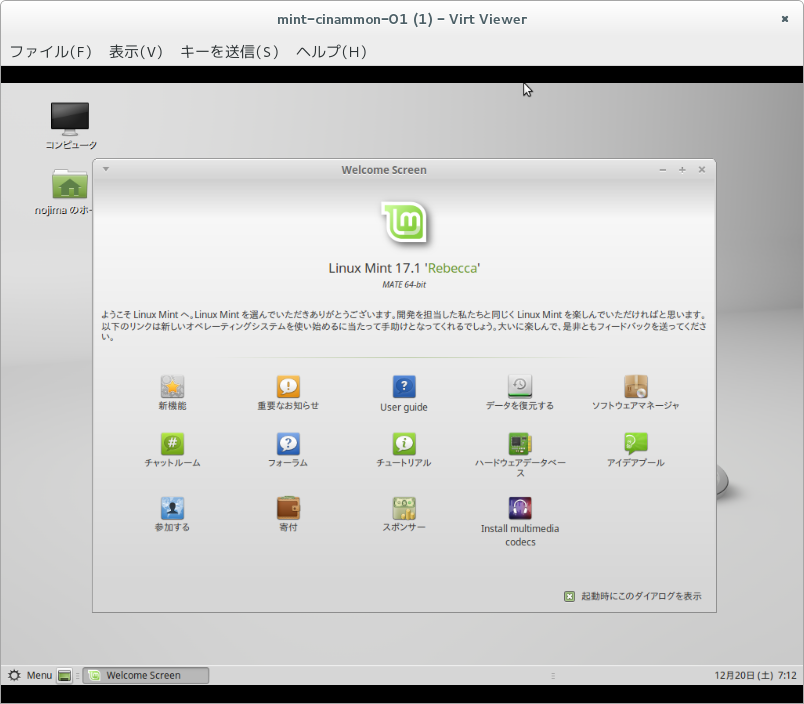
\includegraphics[width=0.7\hsize]{image201412/mint-setupcomplete.png}
\caption{Linux Mint 17.1 のMATE版が動作}
\end{figure}
\end{frame}

\begin{frame}{動かなかった!}

  Linux Mint 17.1のcinnamon版はdebian sidのKVMの元では、cirrus/qxl共に動作が不安定で使えなかったです...orz。
  \begin{center}
   {\LARGE 将来に期待!}
  \end{center}
  
\end{frame}

\begin{frame}{ちょっとだけハマりポイント}

\begin{itemize}
\item virt-viewerで画面描画がおかしい場合は、cirrusの代わりにqxlをvirt側のxml設定ファイルに記述すると非常に良くなる事があります。
\item 音が無くて寂しい場合は、ac97を指定して、vncプロトコルの代わりにspiceプロトコルを指定すると、virt-viewerから音が出ます。
\item ディスクは最低でも9GBytes以上、メモリは1GBytes以上割り当てないとインストールに失敗します。(マニュアルに明記が無いのでハマります)
\end{itemize}
  
\end{frame}

\begin{frame}[containsverbatim]{ちょっとだけハマりポイント}

 仮想側のsoundデバイスを指定し、qxlをビデオドライバに指定して、spiceプロトコルを有効にする設定の例:
  
\begin{commandlinesmall}
$ sudo virt edit mint-01
...xmlファイル中...
 <graphics type='spice' port='5900' autoport='no'>
   <mouse mode='server'/>
   <clipboard copypaste='yes'/>
 </graphics>
 <sound model='ac97'>
 </sound>
 <video>
   <model type='qxl' ram='65536' vram='65536' heads='1'>
     <acceleration accel3d='yes' accel2d='yes'/>
   </model>
 </video>
...xmlファイル中...
\end{commandlinesmall}

\end{frame}


\begin{frame}{参考:コード名}

  Linux Mint はコード名に頭文字がA-Zの順番で決まる女性の名前を使うんだそうです。
 前回のバージョンLinux Mint 17はOiana。今回の最新バージョン17.1はRebbeca。\\
  参考:Debianはトイ・ストーリーのキャラクタ名。

\end{frame}

\begin{frame}{参考:日本語IMは?}

 今までLinux Mintの日本語IM導入はLinux Mint Japanチームの追加パッケージを別途導入しなければなりませんでしたが、Linux Mint 17.1からはログイン後のメニューから、「設定」→「Languages」で起動するユーティリティでメニューから簡単設定出来るようになった模様です。
  
\end{frame}

\begin{frame}{参考:日本語IMは?}

 \begin{figure}[H]
\centering
 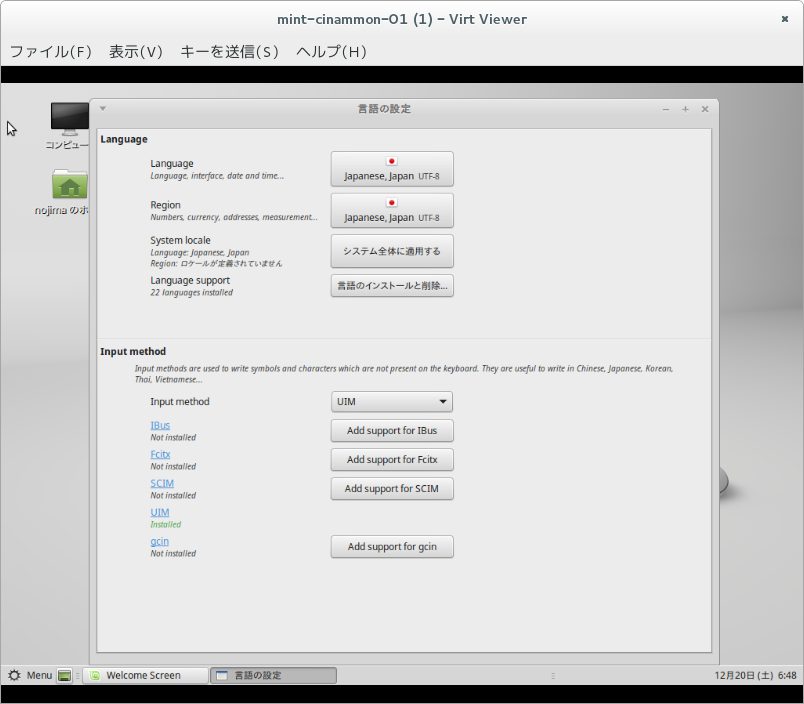
\includegraphics[width=0.7\hsize]{image201412/mint-im-setup.png}
\caption{Linux Mint 17.1 の日本語IM設定/導入メニュー}
\end{figure}
  
\end{frame}

\begin{frame}{Linux MintとUbuntu/Debianの関係}

\begin{figure}[H]
\centering
\includegraphics[width=0.7\hsize]{image201412/mint-construct.eps}
\caption{Linux MintとUbuntu/Debianの関係}
\end{figure}
  
\end{frame}

\begin{frame}{使ってわかるLinux Mintの良さ}

\begin{itemize}
\item Linux Mint側でメンテナンスされている部分の作りが非常に丁寧。GUIとシステム連携の完成度が高い。
 \item Linux Mint側のcommunityサイトは、投票システムを搭載しており、ユーザの投稿のランキングなどの様々な統計がすぐわかる。アイデア投稿もあり、アイデアはすぐに他ユーザの手により評価される。
\end{itemize}
\end{frame}

\begin{frame}{Debianにcinnamon}

  Debianにcinnamon入れたらひょっとしてLinux Mintになる?\\
  wktk...
 
\end{frame}  

\begin{frame}[containsverbatim]{Debianにcinnamon}

\begin{description}
\item [Step 1.] Debian sidをデスクトップ環境を全く導入しない最小限の構成で導入。
\item [Step 2.] cinnamonデスクトップ環境を導入。
  \begin{commandlinesmall}
$ sudo aptitude install cinnamon-desktop-envirionment
  \end{commandlinesmall}
\end{description}

\begin{center}
\LARGE とっても簡単!
\end{center}
\end{frame}  

\begin{frame}{Debianにcinnamon}

できた!

\begin{figure}[H]
\centering
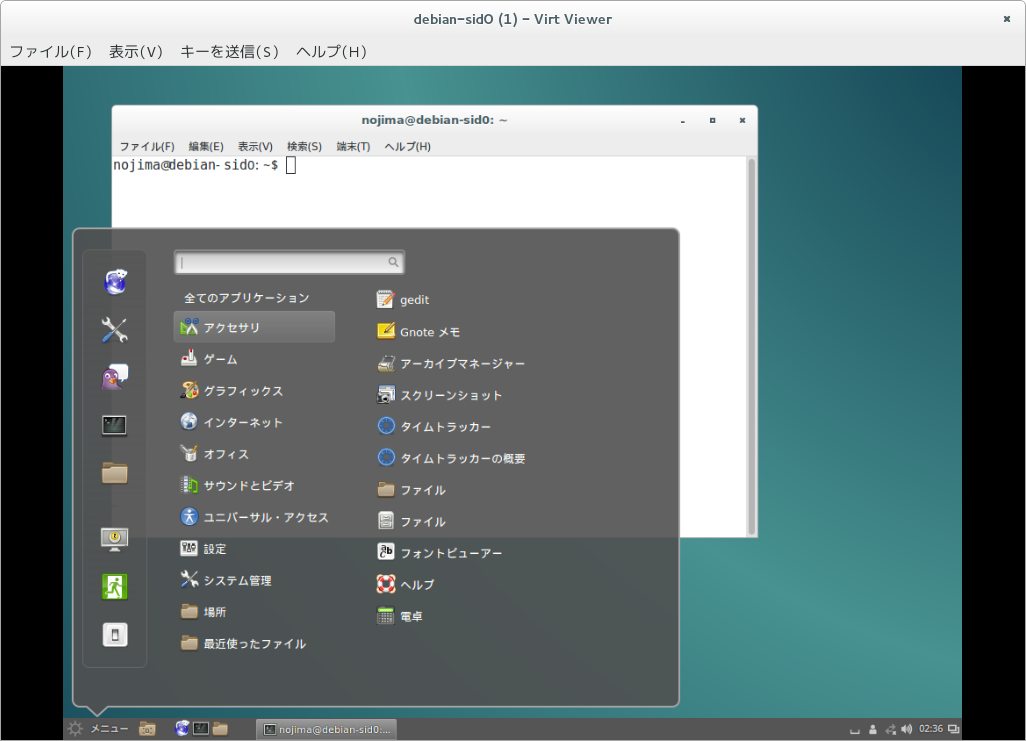
\includegraphics[width=0.6\hsize]{image201412/debian-cinnamon.png}  
\caption{Debianにcinnamonを導入}\label{fig:debian-cinnamon}
\end{figure} 
  
\end{frame}  

\begin{frame}{Debianにcinnamon感想}

  \begin{itemize}
  \item やっぱりDebianのルックアンドフィール。
  \item 考え方もDebianの他のデスクトップ環境と同じポリシー。
  \item OS側との連携度合いも、Debian流。
  \end{itemize}
  
\end{frame}  

\begin{frame}{Debianにcinnamon感想}

  \centering
  うーん、Linux MintをDebianに引き込むにはcinnamonだけじゃダメか...
  
\end{frame}  

\begin{frame}{まとめ}

 Linux Mintの良いところである、
  
\begin{itemize}  
\item Linux Mint communityのサイト(WEB上の投票システムとか、アイデア出しとか)
\item Linux Mint並にGUIとシステム管理が丁寧に統合されたデスクトップ環境の構成
\end{itemize}

はDebianを考えるときに参考になりました!

\end{frame}  

\section{今後のイベント}
\emtext{今後のイベント}
\begin{frame}{今後のイベント}
\begin{itemize}
 \item 関西エリアDebian勉強会
 \item 東京エリアDebian勉強会 
\end{itemize}
\end{frame}

\section{今日の宴会場所}
\emtext{今日の宴会場所}
\begin{frame}{今日の宴会場所}
未定
\end{frame}

\end{document}

;;; Local Variables: ***
;;; outline-regexp: "\\([ 	]*\\\\\\(documentstyle\\|documentclass\\|emtext\\|section\\|begin{frame}\\)\\*?[ 	]*[[{]\\|[]+\\)" ***
;;; End: ***
